\documentclass[11pt]{article}
\usepackage[a4paper,margin=2.4cm]{geometry}
\usepackage{booktabs,graphicx,amsmath,hyperref,xcolor,textcomp}
\hypersetup{colorlinks,linkcolor=blue!50!black,citecolor=blue!50!black,urlcolor=blue!50!black}
\usepackage[numbers,sort&compress]{natbib}

\title{Pennies and Pounds:\\
\large How Common Simplifications of UK Payroll Arithmetic Diverge from HMRC's Exact Method}
\author{Mithil Nagabathula\\University of East London\\\texttt{mithilnishu2000@gmail.com}}
\date{October 2026}

\begin{document}
\maketitle

\begin{abstract}
UK employers must deduct income tax, National Insurance and student loan repayments exactly as HM Revenue and Customs specifies,
including where to round and to what. Payroll code often takes shortcuts: binary floating point, a threshold divided from an annual
figure, a rounding mode chosen by default. We measure the effect of nine such shortcuts, each changing one rule, by differential testing
against an exact-arithmetic reference implementation that reproduces HMRC's worked examples. Over a synthetic workforce of 100{,}000
employees and 2.0 million payslips in tax year 2026--27, floating point alone changed 0.24\% of payslips, concentrated in weekly payroll,
and the cumulative method corrected almost all of these by year end. Other shortcuts were systematic: dividing annual National Insurance
thresholds instead of using HMRC's published period figures changed 88\% of payslips and over-deducted \pounds55{,}556 across the
workforce; rounding student loan repayments to the penny instead of down to the pound over-deducted \pounds159{,}610 and affected 16\% of
employees by \pounds1 or more; skipping the rounding of taxable pay to whole pounds changed 91\% of payslips. Applying the
non-cumulative basis to everyone moved deductions for 73\% of employees by \pounds1 or more, by up to \pounds744. The rules that look
like pedantry are where the money is; floating point, often blamed, mattered least.
\end{abstract}

\section{Introduction}
HMRC's specification for PAYE tax table routines \cite{hmrc2026spec} prescribes not only the tax bands but also every rounding step: taxable
pay to date is rounded down to whole pounds before the tax formula, band limits are pro-rated and truncated to four decimal places, free
pay for codes above 500 uses a quotient method with HMRC's own figures, and tax is rounded down to the penny. National Insurance (NI) uses
thresholds that HMRC publishes per pay period and rounds an exact half penny down \cite{hmrc2026rates}. Student loan repayments are
rounded down to the whole pound \cite{hmrc2026sl}.

Each of these rules is easy to get slightly wrong, and payroll code is often written from a general description of the tax rather
than the specification. The usual suspicion falls on binary floating point \cite{goldberg1991,ieee754}. We ask a more useful question:
which simplifications actually change what employees are paid, how often and by how much?

We answer it by differential testing \cite{mckeeman1998}. The reference is an open-source engine that implements HMRC's exact
percentage method in rational arithmetic and passes HMRC's published worked examples \cite{payrollengine}. Each shortcut is a separate
implementation that differs from the reference in exactly one rule, and all are run on the same randomised workforce, in the spirit of
property-based testing \cite{claessen2000quickcheck}.

\section{Method}
\paragraph{Reference.} The engine computes PAYE by HMRC's exact percentage method (specification v24.0 for 2026--27), Class 1 NI by
category, and student loan deductions, with money held as integer pence and all intermediate values as exact rationals. Its test suite
reproduces HMRC's worked examples, including monthly free pay of \pounds1{,}048.26 for code 1257L and \pounds19.41 weekly additional pay
for K100.

\paragraph{Workforce.} 100{,}000 employees, 80\% paid monthly and 20\% weekly, with annual pay drawn from a lognormal distribution with
median \pounds37{,}000 and log-standard deviation 0.55 (floored near \pounds6{,}000). 30\% have pay that varies by \(\pm5\%\) per
period and 15\% receive a bonus equal to one period's pay. Tax codes: 80\% 1257L, 8\% Scottish S1257L, 3\% Welsh C1257L, 3\% BR, 3\% K
codes (K50--K649) and 3\% other allowance codes (600L--1999L); 4\% of codes are on a Week 1/Month 1 basis. NI categories are A, with
5\% M (under 21) and 3\% C (over State Pension age); 24\% repay a student loan (plans 1, 2, 4 or 5). The workforce is generated with a
fixed seed and run through all 52 or 12 periods of the tax year, giving 2{,}003{,}080 payslips.

\paragraph{Shortcuts.} Six PAYE variants (floating point; band limits pro-rated without truncation or the income-test ceiling; no
rounding of taxable pay to whole pounds; no quotient method; rounding tax to the nearest penny; the non-cumulative basis for everyone),
two NI variants (half-up rounding; thresholds computed as annual/periods) and one student loan variant (penny rather than pound
rounding). All PAYE variants except the first also use floating point, so their effects include the first's; all apply HMRC's 50\%
regulatory limit as the reference does.

\paragraph{Measures.} For each shortcut: the share of payslips whose deduction differs from the reference, the largest single
difference, the share of employees whose annual total differs at all and by \pounds1 or more, the largest annual difference, and the
net difference summed across the workforce.

\section{Results}
\begin{table*}[t]
\centering
\caption{Differences from HMRC's exact method for 100,000 employees and 2,003,080 payslips over tax year 2026-27. Each shortcut changes one rule. Net is the sum over all employees of (shortcut $-$ exact) annual deductions; positive means over-deduction.}
\label{tab:main}
\footnotesize
\setlength{\tabcolsep}{3pt}
\begin{tabular}{p{6.2cm}rrrrrr}
\toprule
Shortcut & Slips $\neq$ & Max/slip & Staff $\neq$ & Staff $\geq$\pounds1 & Max/year & Net \\
\midrule
PAYE: Exact algorithm in binary floating point & 0.24\% & \pounds0.48 & 0.11\% & 0.00\% & \pounds0.42 & $-$\pounds24 \\
PAYE: Band limits pro-rated without truncation or ceiling & 0.59\% & \pounds0.48 & 0.11\% & 0.00\% & \pounds0.42 & $-$\pounds24 \\
PAYE: Taxable pay not rounded down to whole pounds & 90.65\% & \pounds0.48 & 89.37\% & 2.84\% & \pounds22.36 & \pounds21,108 \\
PAYE: Free pay without the quotient method & 19.84\% & \pounds0.48 & 17.99\% & 0.02\% & \pounds20.80 & \pounds4,808 \\
PAYE: Tax rounded to nearest penny, not down & 14.00\% & \pounds0.49 & 1.26\% & 0.00\% & \pounds0.52 & \pounds102 \\
PAYE: Week 1/Month 1 basis for everyone & 50.34\% & \pounds739.46 & 91.10\% & 72.93\% & \pounds743.66 & \pounds1,925,374 \\
NI: Half a penny rounded up, not down & 0.50\% & \pounds0.01 & 2.87\% & 0.00\% & \pounds0.52 & \pounds101 \\
NI: Thresholds as annual/periods, not HMRC's figures & 87.82\% & \pounds0.05 & 93.33\% & 13.23\% & \pounds1.56 & \pounds55,556 \\
Student loan: Rounded down to the penny, not the pound & 16.04\% & \pounds0.99 & 17.22\% & 15.59\% & \pounds51.48 & \pounds159,610 \\
\bottomrule
\end{tabular}
\end{table*}


Table~\ref{tab:main} and Figure~\ref{fig:emp} summarise the results. They fall into three groups.

\paragraph{Floating point: rare and self-correcting.} Running HMRC's algorithm in binary floating point changed 0.24\% of payslips, by up
to 48p. Every difference we inspected arose when taxable pay to date landed exactly on a whole pound: the exact value rounds down to
itself, while the floating-point value, a hair below, rounds down to the pound before, which at 20\% is 20p of tax. The effect was
concentrated in weekly payroll (0.55\% of weekly employees ended the year with a different total, against 0.004\% of monthly employees),
and the cumulative method repaired almost all of it the following period. Only 0.11\% of employees ended the year with a different total,
by at most 42p.

\paragraph{Systematic shortcuts: small per payslip, large in aggregate.} Three shortcuts changed most payslips by a few pence in the same
direction. Not rounding taxable pay down to whole pounds changed 91\% of payslips and left 2.8\% of employees at least \pounds1 out at
year end. Computing NI thresholds as annual figures divided by the number of periods (for example a monthly primary threshold of
\pounds1{,}047.50 instead of HMRC's \pounds1{,}048) changed 88\% of payslips by up to 5p, over-deducting \pounds55{,}556 across the
workforce in a year. Omitting the quotient method shifted free pay by a penny per period for most codes and by more for large code
numbers. Each is the kind of difference a payslip check against a calculator would dismiss, and each is a breach of the specification
on almost every payslip.

\paragraph{Rules with real money attached.} Rounding student loan deductions down to the penny instead of the pound over-deducted up to
99p per payslip and \pounds51.48 per employee per year, and \pounds159{,}610 in total. Applying the Week 1/Month 1 basis to everyone, a
simplification sometimes made when cumulative data are unavailable, moved annual deductions for 73\% of employees by \pounds1 or more:
the median employee was under-deducted \pounds1.20, while those with a bonus month were over-deducted by up to \pounds744, because the
non-cumulative basis cannot spread a bonus across the year's allowances.

\begin{figure}[t]
  \centering
  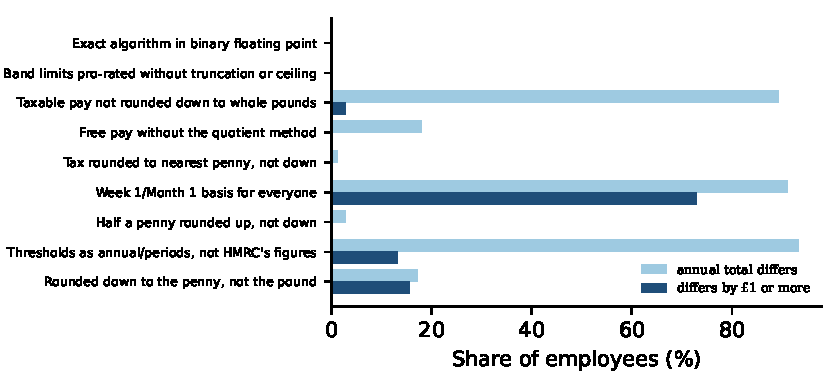
\includegraphics[width=0.85\linewidth]{figures/employees.pdf}
  \caption{Share of employees whose annual deductions differ from the exact method, at all and by \pounds1 or more.}
  \label{fig:emp}
\end{figure}

\section{Discussion}
The findings invert a common intuition. Floating point, the usual suspect, was the least consequential shortcut, because PAYE is
cumulative and corrects itself. The shortcuts that matter are rules that look like pedantry: which threshold table to use, which rounding
unit, which basis. They are invisible on a single payslip and systematic across a workforce, which is the worst combination for detection.

For implementers we draw three lessons. (1) Use HMRC's published period figures, never a derived division. (2) Keep money in integer
pence and intermediate values exact, not because floating point is often wrong but because it makes every other rule harder to reason
about. (3) Test against a reference implementation over a realistic population, not only against HMRC's handful of worked examples,
which every shortcut here except the non-cumulative basis would pass on most inputs.

\paragraph{Limitations.} The workforce is synthetic; real pay distributions, tax-code mixes and pay patterns differ and would change the
magnitudes. Each shortcut was tested alone; real systems may combine several, and effects can interact. The reference implementation is
the author's own and is validated against HMRC's worked examples and tables, not against HMRC's own software. We did not examine
pensions, statutory payments or salary sacrifice.

\section{Conclusion}
Across two million simulated payslips, the simplifications that most changed UK payroll deductions were rounding and threshold rules,
not floating-point arithmetic. Payroll software should be tested differentially against an exact reference over a realistic workforce.

\paragraph{Reproducibility.} The simulation runs in under a minute; code and results will be released at
\newline\url{https://github.com/mithil2k2000-tech/payroll-shortcuts}.

\paragraph{Use of AI tools.} An AI assistant (Claude, Anthropic) helped write code for the engine and this study and draft text. The
author designed the study, reviewed the code and results, and takes responsibility for the content.

\bibliographystyle{plainnat}
\bibliography{refs}
\end{document}
